

\tikzset{every picture/.style={line width=0.75pt}} %set default line width to 0.75pt        

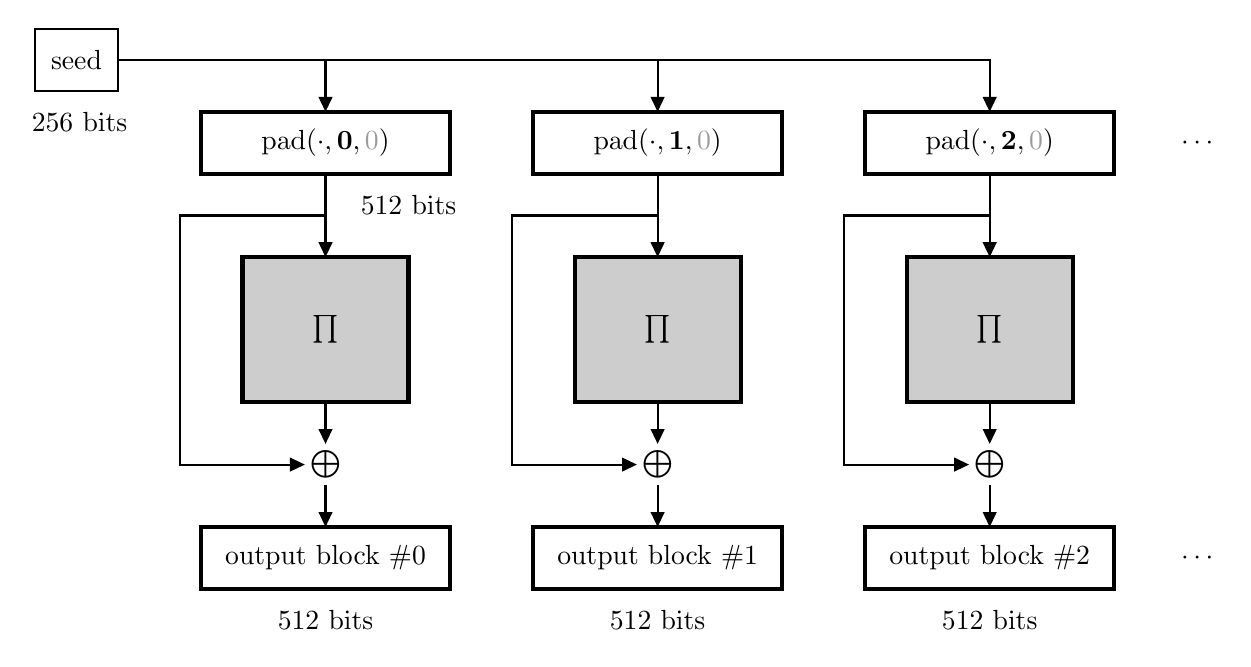
\begin{tikzpicture}[x=0.75pt,y=0.75pt,yscale=-1,xscale=1]
%uncomment if require: \path (0,308); %set diagram left start at 0, and has height of 308

%Shape: Rectangle [id:dp4230275453277854] 
\draw  [fill={rgb, 255:red, 155; green, 155; blue, 155 }  ,fill opacity=0.5 ][line width=1.5]  (100,110) -- (180,110) -- (180,180) -- (100,180) -- cycle ;
%Shape: Rectangle [id:dp9132465255651376] 
\draw  [line width=1.5]  (80,40) -- (200,40) -- (200,70) -- (80,70) -- cycle ;
%Shape: Rectangle [id:dp9442325704085703] 
\draw  [fill={rgb, 255:red, 155; green, 155; blue, 155 }  ,fill opacity=0.5 ][line width=1.5]  (260,110) -- (340,110) -- (340,180) -- (260,180) -- cycle ;
%Shape: Rectangle [id:dp6369888587529804] 
\draw  [line width=1.5]  (240,40) -- (360,40) -- (360,70) -- (240,70) -- cycle ;
%Shape: Rectangle [id:dp699706499450861] 
\draw  [fill={rgb, 255:red, 155; green, 155; blue, 155 }  ,fill opacity=0.5 ][line width=1.5]  (420,110) -- (500,110) -- (500,180) -- (420,180) -- cycle ;
%Shape: Rectangle [id:dp7715907441243712] 
\draw  [line width=1.5]  (400,40) -- (520,40) -- (520,70) -- (400,70) -- cycle ;
%Shape: Rectangle [id:dp7734942875538231] 
\draw  [line width=0.75]  (0,0) -- (40,0) -- (40,30) -- (0,30) -- cycle ;
%Straight Lines [id:da8996997470966899] 
\draw    (40,15) -- (460,15) -- (460,37) ;
\draw [shift={(460,40)}, rotate = 270] [fill={rgb, 255:red, 0; green, 0; blue, 0 }  ][line width=0.08]  [draw opacity=0] (7.14,-3.43) -- (0,0) -- (7.14,3.43) -- cycle    ;
%Straight Lines [id:da04557569134913253] 
\draw    (300,15) -- (300,37) ;
\draw [shift={(300,40)}, rotate = 270] [fill={rgb, 255:red, 0; green, 0; blue, 0 }  ][line width=0.08]  [draw opacity=0] (7.14,-3.43) -- (0,0) -- (7.14,3.43) -- cycle    ;
%Straight Lines [id:da9963128750519981] 
\draw    (140,15) -- (140,37) ;
\draw [shift={(140,40)}, rotate = 270] [fill={rgb, 255:red, 0; green, 0; blue, 0 }  ][line width=0.08]  [draw opacity=0] (7.14,-3.43) -- (0,0) -- (7.14,3.43) -- cycle    ;
%Straight Lines [id:da5456800515951024] 
\draw    (140,70) -- (140,107) ;
\draw [shift={(140,110)}, rotate = 270] [fill={rgb, 255:red, 0; green, 0; blue, 0 }  ][line width=0.08]  [draw opacity=0] (7.14,-3.43) -- (0,0) -- (7.14,3.43) -- cycle    ;
%Straight Lines [id:da3695926238160996] 
\draw    (300,70) -- (300,107) ;
\draw [shift={(300,110)}, rotate = 270] [fill={rgb, 255:red, 0; green, 0; blue, 0 }  ][line width=0.08]  [draw opacity=0] (7.14,-3.43) -- (0,0) -- (7.14,3.43) -- cycle    ;
%Straight Lines [id:da6798756598406426] 
\draw    (460,70) -- (460,107) ;
\draw [shift={(460,110)}, rotate = 270] [fill={rgb, 255:red, 0; green, 0; blue, 0 }  ][line width=0.08]  [draw opacity=0] (7.14,-3.43) -- (0,0) -- (7.14,3.43) -- cycle    ;
%Straight Lines [id:da04652918034563491] 
\draw    (140,180) -- (140,197) ;
\draw [shift={(140,200)}, rotate = 270] [fill={rgb, 255:red, 0; green, 0; blue, 0 }  ][line width=0.08]  [draw opacity=0] (7.14,-3.43) -- (0,0) -- (7.14,3.43) -- cycle    ;
%Straight Lines [id:da4795698833977069] 
\draw    (300,180) -- (300,197) ;
\draw [shift={(300,200)}, rotate = 270] [fill={rgb, 255:red, 0; green, 0; blue, 0 }  ][line width=0.08]  [draw opacity=0] (7.14,-3.43) -- (0,0) -- (7.14,3.43) -- cycle    ;
%Straight Lines [id:da6614845169362173] 
\draw    (460,180) -- (460,197) ;
\draw [shift={(460,200)}, rotate = 270] [fill={rgb, 255:red, 0; green, 0; blue, 0 }  ][line width=0.08]  [draw opacity=0] (7.14,-3.43) -- (0,0) -- (7.14,3.43) -- cycle    ;
%Straight Lines [id:da2537084726269978] 
\draw    (140,220) -- (140,237) ;
\draw [shift={(140,240)}, rotate = 270] [fill={rgb, 255:red, 0; green, 0; blue, 0 }  ][line width=0.08]  [draw opacity=0] (7.14,-3.43) -- (0,0) -- (7.14,3.43) -- cycle    ;
%Straight Lines [id:da08364635273503662] 
\draw    (300,220) -- (300,237) ;
\draw [shift={(300,240)}, rotate = 270] [fill={rgb, 255:red, 0; green, 0; blue, 0 }  ][line width=0.08]  [draw opacity=0] (7.14,-3.43) -- (0,0) -- (7.14,3.43) -- cycle    ;
%Straight Lines [id:da8323517004914498] 
\draw    (460,220) -- (460,237) ;
\draw [shift={(460,240)}, rotate = 270] [fill={rgb, 255:red, 0; green, 0; blue, 0 }  ][line width=0.08]  [draw opacity=0] (7.14,-3.43) -- (0,0) -- (7.14,3.43) -- cycle    ;
%Straight Lines [id:da4039327675118729] 
\draw    (140,90) -- (70,90) -- (70,210) -- (127,210) ;
\draw [shift={(130,210)}, rotate = 180] [fill={rgb, 255:red, 0; green, 0; blue, 0 }  ][line width=0.08]  [draw opacity=0] (7.14,-3.43) -- (0,0) -- (7.14,3.43) -- cycle    ;
%Straight Lines [id:da336610285093796] 
\draw    (300,90) -- (230,90) -- (230,210) -- (287,210) ;
\draw [shift={(290,210)}, rotate = 180] [fill={rgb, 255:red, 0; green, 0; blue, 0 }  ][line width=0.08]  [draw opacity=0] (7.14,-3.43) -- (0,0) -- (7.14,3.43) -- cycle    ;
%Straight Lines [id:da9191028994452097] 
\draw    (460,90) -- (390,90) -- (390,210) -- (447,210) ;
\draw [shift={(450,210)}, rotate = 180] [fill={rgb, 255:red, 0; green, 0; blue, 0 }  ][line width=0.08]  [draw opacity=0] (7.14,-3.43) -- (0,0) -- (7.14,3.43) -- cycle    ;
%Shape: Rectangle [id:dp5078655301930546] 
\draw  [line width=1.5]  (80,240) -- (200,240) -- (200,270) -- (80,270) -- cycle ;
%Shape: Rectangle [id:dp17401855535242738] 
\draw  [line width=1.5]  (240,240) -- (360,240) -- (360,270) -- (240,270) -- cycle ;
%Shape: Rectangle [id:dp2688302867140522] 
\draw  [line width=1.5]  (400,240) -- (520,240) -- (520,270) -- (400,270) -- cycle ;

% Text Node
\draw (140,145) node    {$\prod $};
% Text Node
\draw (140,55) node    {$\mathrm{pad}( \cdot ,\mathbf{0} ,\textcolor[rgb]{0.61,0.61,0.61}{0})$};
% Text Node
\draw (300,145) node    {$\prod $};
% Text Node
\draw (300,55) node    {$\mathrm{pad}( \cdot ,\mathbf{1} ,\textcolor[rgb]{0.61,0.61,0.61}{0})$};
% Text Node
\draw (460,145) node    {$\prod $};
% Text Node
\draw (460,55) node    {$\mathrm{pad}( \cdot ,\mathbf{2} ,\textcolor[rgb]{0.61,0.61,0.61}{0})$};
% Text Node
\draw (20,15) node   [align=left] {seed};
% Text Node
\draw (140,210) node    {$\bigoplus $};
% Text Node
\draw (300,210) node    {$\bigoplus $};
% Text Node
\draw (460,210) node    {$\bigoplus $};
% Text Node
\draw (140,255) node   [align=left] {output block \#$\displaystyle 0$};
% Text Node
\draw (300,255) node   [align=left] {output block \#$\displaystyle 1$};
% Text Node
\draw (460,255) node   [align=left] {output block \#$\displaystyle 2$};
% Text Node
\draw (180,85) node   [align=left] {$\displaystyle 512$ bits};
% Text Node
\draw (140,285) node   [align=left] {$\displaystyle 512$ bits};
% Text Node
\draw (300,285) node   [align=left] {$\displaystyle 512$ bits};
% Text Node
\draw (460,285) node   [align=left] {$\displaystyle 512$ bits};
% Text Node
\draw (560,55) node   [align=left] {$\displaystyle \cdots $};
% Text Node
\draw (560,255) node   [align=left] {$\displaystyle \cdots $};
% Text Node
\draw (-3,45) node [anchor=west] [inner sep=0.75pt]   [align=left] {$\displaystyle 256$ bits};


\end{tikzpicture}